\section{تراکنش}

تراکنش واحد اجرای برنامه است. عملیاتی که در هر تراکنش می‌تواند شامل شود موارد
زیر می‌باشد:

\begin{itemize}
    \item Create
    \item Read
    \item Update
    \item Delete
\end{itemize}

\section{قوانین \lr{ACID}}

\subsection{اتمیک یا \lr{Atomicity}}

هر تراکنش دیتابیس به صورت اتمیک می‌باشد. این قضیه بدان معناست که این تراکنش یا
باید کاملا انجام شود یا کلا لغو و صرف نظر شود. در غیر این صورت اگر تراکنش به
صورت ناتمام و ناقص انجام شود عواقب مختلفی روی دیتابیس خواهد گذاشت.

\subsection{جامعیت یا \lr{Consistency}}

هر تراکنش باید از قوانین جامعیت پیروی کند. نمی‌توان داده‌ای را وارد جدولی از
دیتابیس کرد که به صورت معتبر نباشد. در برخی از مراجع این قانون را به اجرای صحیح
و سازگار تراکنش می‌شناسند. مهم ترین مثال آن است که شما یک \lr{Validation} روی یک
مقداری از فیلد جدول تنظیم می‌کنید که هر داده‌ای بر روی آن فقط با شرایط تعریف شده
بایستی وارد شود.

مرجع پذیری زمانی مطرح می‌شود که یک رکوردی از داده وقتی وارد جدولی از دیتابیس
می‌شود ممکن است ارتباط مشخصی با جدولی دیگر داشته باشد. پس به همین خاطر کلید‌های
اصلی و خارجی در خصوص جامعیت وجود دارند که داده‌ای معنادار را پس از پرس و جو از
دیتابیس به برنامه نویس برگرداند (یادآوری، بخش جوین‌ها در دیتابیس و تعریف رفرنس
در هنگام تعریف کلید جانبی).

\subsection{انزوا یا \lr{Isolation}}

هر سیستم جامع پایگاه داده‌ای باید بتواند روی همروندی تراکنش‌ها مدیریت و کنترل
کامل داشته باشد. انزوا تراکنش‌ها قابلیت کنترل و تنظیم بر اساس \lr{DBMS} است. به
طور کل همروندی یا همزمانی به حالتی گفته می‌شود که چند تراکنش بخواهند در یک زمان
به صورت موازی روی یک منبع عملیات خواندن و نوشتن را انجام دهند. اما این عملیات به
طور کل هزینه خاص و مشخصی برای برنامه نویس و مدیر دیتابیس دارد.

\subsection{قابلیت اعتماد یا \lr{Duribility}}

قابلیت اعتماد یکی از مهم‌ترین ویژگی‌های هر سیستم دیتابیسی است. یعنی بتوان
داده‌ها را در پایگاه‌داده به صورت پایدار و ثابت نگهداری و مراقبت کرد. در صورت
بروز مشکل روی داده‌های یک دیتابیس می‌توان به عملیات انجام شده در این قسمت مراجعه
کرد. بطور کلی این بخش قابلیت کنترل و مدیریت دارد و می‌توان مجموعه فرایند‌های
نگهداری و بک‌آپ را به صورت خودکار انجام داد.

\newpage

\subsection{تنظیم قابلیت انزوا}

انزوا و مدیریت همروندی در دیتابیس به چهار طریق قابل انجام است:

\begin{enumerate}
    \item \lr{Read uncommitted}
    \item \lr{Read commmitted} 
    \item \lr{Repeadable read}
    \item \lr{Serializable}
\end{enumerate}

یادآوری: هر تراکنش دو حالت در پایان پیدا می‌کند:

\begin{itemize}
    \item \lr{Commit}: تراکنش درنهایت تایید و انجام می‌شود
    \item \lr{Abort}: تراکنش در نهایت ساقط یا صرفه نظر می‌شود
\end{itemize}

\subsubsection{وضعیت تراکنش}

نکته: \lr{Abort} در دو شرط اتفاق می‌افتد:

\begin{enumerate}
    \item زمانی که اجرای تراکنش به خطای \lr{Runtime} دچار شود.
    \item خرابی و نقص سیستم که روی اجرای تراکنش تاثیر می‌گذارد که کامل نشود
\end{enumerate}

\begin{figure}[H]
    \centering
    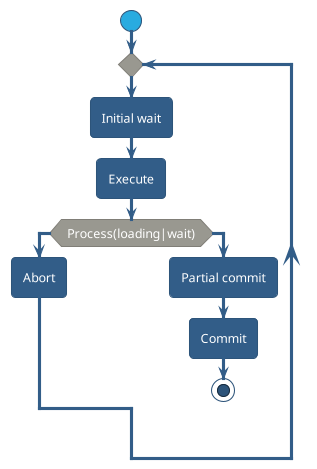
\includegraphics[width=0.4\textwidth]{umls/transactionStatus.png}
    \caption{نمودار شروع فرایند تراکنش‌ها}
    \label{fig: uml}
\end{figure}

\newpage